\begin{table*}[!htp]
\begin{center}
\small
 \begin{tabular}{|l|c|c|c|c|c|c|c|c|c|}
  \hline
Event & IDT\cite{Wang_CVPR11} & IDT\cite{Wang_CVPR11} player & C3D \cite{Tran_arxiv14} & MIL\cite{Andrews_NIPS02} &  LRCN \cite{Donahue_arxiv14} &Only player & Avg. player & Our no track & Our track \\ \hline \hline

  3-point succ.    & 0.370 & 0.428 & 0.117 & 0.237 & 0.462   & 0.469 & 0.545 & 0.583 & \textbf{0.600} \\
  3-point fail.    & 0.501 &  0.481& 0.282 & 0.335 & 0.564   & 0.614 & 0.702 & 0.668 & \textbf{0.738} \\
  fr-throw succ. & 0.778 &  0.703& 0.642   & 0.597 & 0.876   & 0.885 & 0.809 & \textbf{0.892} & 0.882 \\
  fr-throw fail. & 0.365 &  0.623& 0.319   & 0.318 & 0.584    & \textbf{0.700} & 0.641 & 0.671 & 0.516 \\
  layup succ.      & 0.283 & 0.300 & 0.195 & 0.257 & 0.463   & 0.416 & 0.472 & 0.489 & \textbf{0.500} \\
  layup fail.      & 0.278 &0.311  & 0.185 & 0.247 & 0.386   & 0.305 & 0.388 & 0.426 & \textbf{0.445} \\
  2-point succ.    & 0.136 &  0.233 & 0.078& 0.224 & 0.257    & 0.228 & 0.255 & 0.281 & \textbf{0.341} \\
  2-point fail.    & 0.303 &  0.285 & 0.254& 0.299 & 0.378   & 0.391 & \textbf{0.473} & 0.442 & 0.471 \\
  sl. dunk succ.  & 0.197 &  0.171 & 0.047 & 0.112 & 0.285   & 0.107 & 0.186 & 0.210 & \textbf{0.291} \\
  sl. dunk fail.  & 0.004 &  0.010 & 0.004 & 0.005 & \textbf{0.027} & 0.006 & 0.010 & 0.006 & 0.004 \\
  steal            & 0.555 &  0.473& 0.303 & 0.843 & 0.876 &  0.843 & \textbf{0.894} & 0.886 & 0.893 \\ \hline \hline
Mean             & 0.343 &  0.365 & 0.221  & 0.316 & 0.469 & 0.452 & 0.489 & 0.505 & \textbf{0.516} \\ \hline
  \end{tabular}
\end{center}
  \caption{Mean average precision for event {\em classification} given
    isolated clips.}
  \label{tab:event_class}
  \label{tab:class_res}
\end{table*}


\begin{table*}[ht!]
\begin{center}
\small
 \begin{tabular}{|l|c|c|c|c|c|c|c|c|}
  \hline
Event & IDT\cite{Wang_CVPR11} & IDT player\cite{Wang_CVPR11} & C3D \cite{Tran_arxiv14} & LRCN \cite{Donahue_arxiv14} & Only player & Avg. player & Attn no track & Attn track \\ \hline \hline
3-point succ.    & 0.194  & 0.203 &  0.123 & 0.230 & 0.251 & \textbf{0.268} & 0.263 & 0.239 \\
3-point fail.    & 0.393  & 0.376 &  0.311 & 0.505 & 0.526 & 0.521 & 0.556 & \textbf{0.600} \\
free-throw succ. & 0.585  & 0.621 &  0.542 & 0.741 & 0.777 & \textbf{0.811} & 0.788 & 0.810 \\
free-throw fail. & 0.231  & 0.277 &  0.458 & 0.434 & \textbf{0.470} & 0.444 & 0.468 & 0.405 \\
layup succ.      & 0.258  & 0.290 &  0.175 & 0.492 & 0.402 & 0.489 & 0.494 & \textbf{0.512} \\
layup fail.      & 0.141  & 0.200 &  0.151 & 0.187 & 0.142 & 0.139 & 0.207 & \textbf{0.208} \\
2-point succ.    & 0.161  & 0.170 &  0.126 & 0.352 & 0.371 & \textbf{0.417} & 0.366 & 0.400 \\
2-point fail.    & 0.358  & 0.339 &  0.226 & 0.544 & 0.578 & \textbf{0.684} & 0.619 & 0.674 \\
  slam dunk succ.& 0.137  & 0.275 &  0.114 & 0.428 & 0.566 & 0.457 & 0.576 & \textbf{0.555} \\
slam dunk fail.  & 0.007  & 0.006 &  0.003 & \textbf{0.122} & 0.059 & 0.009 & 0.005 & 0.045 \\
steal            & 0.242  & 0.255 &  0.187 & \textbf{0.359} & 0.348 & 0.313 & 0.340 & 0.339 \\ \hline \hline
Mean             & 0.246  & 0.273 &  0.219 & 0.400 & 0.408 & 0.414 & 0.426 & \textbf{0.435} \\ \hline
  \end{tabular}
\end{center}
  \caption{Mean average precision for event {\em detection} given
    untrimmed videos.}
  \label{tab:detection_res}
\end{table*}

\section{Experimental evaluation}
\label{sec:experiments}

In this section, we present three sets of experiments on the NCAA basketball
dataset: 1. event classification, 2. event detection and 3. evaluation of
attention.

\subsection{Implementation details}

We used a hidden state dimension of $256$ for all the LSTM and BLSTM RNNs, an
embedding layer with ReLU non-linearity and $256$ dimensions for embedding the
player features and frame features before feeding to the RNNs.  We used $32
\times 32$ bins with spatial pyramid pooling for the player location feature.
All the event videos clips were four seconds long and subsampled to 6fps.  The
$\tau$ value was set to $0.25$ for the attention softmax weighting. We used a
batch size of $128$, and a learning rate of $0.005$ which was reduced by a factor of
$0.1$ every $10000$ iterations with RMSProp\cite{RMSProp}. The models were
trained on a cluster of $20$ GPUs for $100k$ iterations over one day.  The
hyperparameters were chosen by cross-validating on the validation set.

\subsection{Event classification}

In this section, we compare the ability of methods to classify isolated
video-clips into 11 classes.  We do not use any additional
negatives from other parts of the basketball videos.  We compare our results
against different control settings and baseline models explained below:

\begin{itemize}\denselist
  \item \emph{IDT\cite{Wang_CVPR11}} We use the publicly available implementation of dense trajectories with
  Fisher encoding.
  
  \item \emph{IDT\cite{Wang_CVPR11} player} We use IDT along with averaged features extracted from the player
  bounding boxes.

  \item \emph{C3D \cite{Tran_arxiv14}} We use the publicly available pre-trained model for feature extraction
  with an SVM classifier.

  \item \emph{LRCN \cite{Donahue_arxiv14}} We use an LRCN model with frame-level features. However, we use
    a BLSTM in place of an LSTM. We found this to improve performance. Also, we do not back-propagate
    into the CNN extracting the frame-level features to be consistent with our model.

  \item \emph{MIL \cite{Andrews_NIPS02}} We use a multi-instance learning
    method to learn bag (frame) labels from the set of player features.

\item \emph{Only player} We only use our player features from Sec.~\ref{sec:feature_extraction} in our model
  without frame-level features.
 
  \item \emph{Avg. player} We combine the player features by simple averaging, without
using  attention.

  \item \emph{Attention no track} Our model without tracks (Eq.~\ref{eq:notrack}).

  \item \emph{Attention with track} Our model with tracking (Eq.~\ref{eq:track}).
\end{itemize}

The mean average precision (mAP) for each setting is shown in Tab.~\ref{tab:class_res}. We see
that the method that uses both global information and local player information
outperforms the model only using local player information (``Only player'') and only
using global information (``LRCN'').  We also show that combining the player
information using a weighted sum (i.e., an attention model) is better than
uniform averaging (``Avg. player''), with the tracking based version of
attention slightly better than the track-free version.  Also, a standard
weakly-supervised approach such as MIL seems to be less effective than any of
our modeling variants.

The performance varies by class.
In particular, performance is much poorer (for all methods) for classes
such as ``slam dunk fail'' for which we have very little data.
However, performance is better for shot-based events like
``free-throw'', ``layups'' and ``3-pointers''where attending to
the shot making person or defenders can be useful. 
\eat{
On the other hand,
``steal'' does not benefit from attention, since it is easy to
distinguish this class from others.
which
is the only event without an attempted shot is easy to distniguish
from the others and does not benefit much from attention.
}

\subsection{Event detection}

In this section, we evaluate the ability of methods to temporally localize
events in untrimmed videos.  We use a sliding window approach, where we slide a
$4$ second window through all the basketball videos and try to classify the
window into a negative class or one of the 11 event classes. We use a stride
length of $2$ seconds.  We treat all windows which do not overlap more than $1$
second with any of the $11$ annotated events as negatives. We use the same setting
for training, test and validation.  This leads to $90200$ negative examples
across all the videos.  We compare with the same baselines as before. However,
we were unable to train the MIL model due to computational limitations.

The detection results are presented in Tab.~\ref{tab:detection_res}.  We see
that, as before, the attention models beat previous state of the art methods.
Not surprisingly, all methods are slightly worse at temporal localization than
for classifying isolated clips.  We also note a significant
difference in classification and detection performance for ``steal" in all
methods.  This can be explained by the large number of negative instances
introduced in the detection setting. These negatives often correspond to
players passing the ball to each other. The ``steal" event is quite similar to
a ``pass" except that the ball is passed to a player of the opposing team. This
makes the ``steal" detection task considerably more challenging.

\subsection{Analyzing attention}

We have seen above that attention can improve the performance of the
model at tasks such as classification and detection. 
Now, we evaluate how accurate the attention models are at
identifying the key players. (Note that the models were never
explicitly trained to identify key players).

\eat{
While attention to specific players improves event detection,
the attention scores themselves carry valuable information.
We observed that the attention scores represented a 
consistent meaning across multiple videos in our dataset.
More concretely, our model often ``attends" to the person shooting the
ball at the beginning of an event. We can see several visual examples
in Fig.~\ref{fig:visual_attention}, where the person shooting
the ball is highlighted by attention.}


% -------- Heat Map for youtube videos
\begin{figure*}[t!]
\begin{center}
   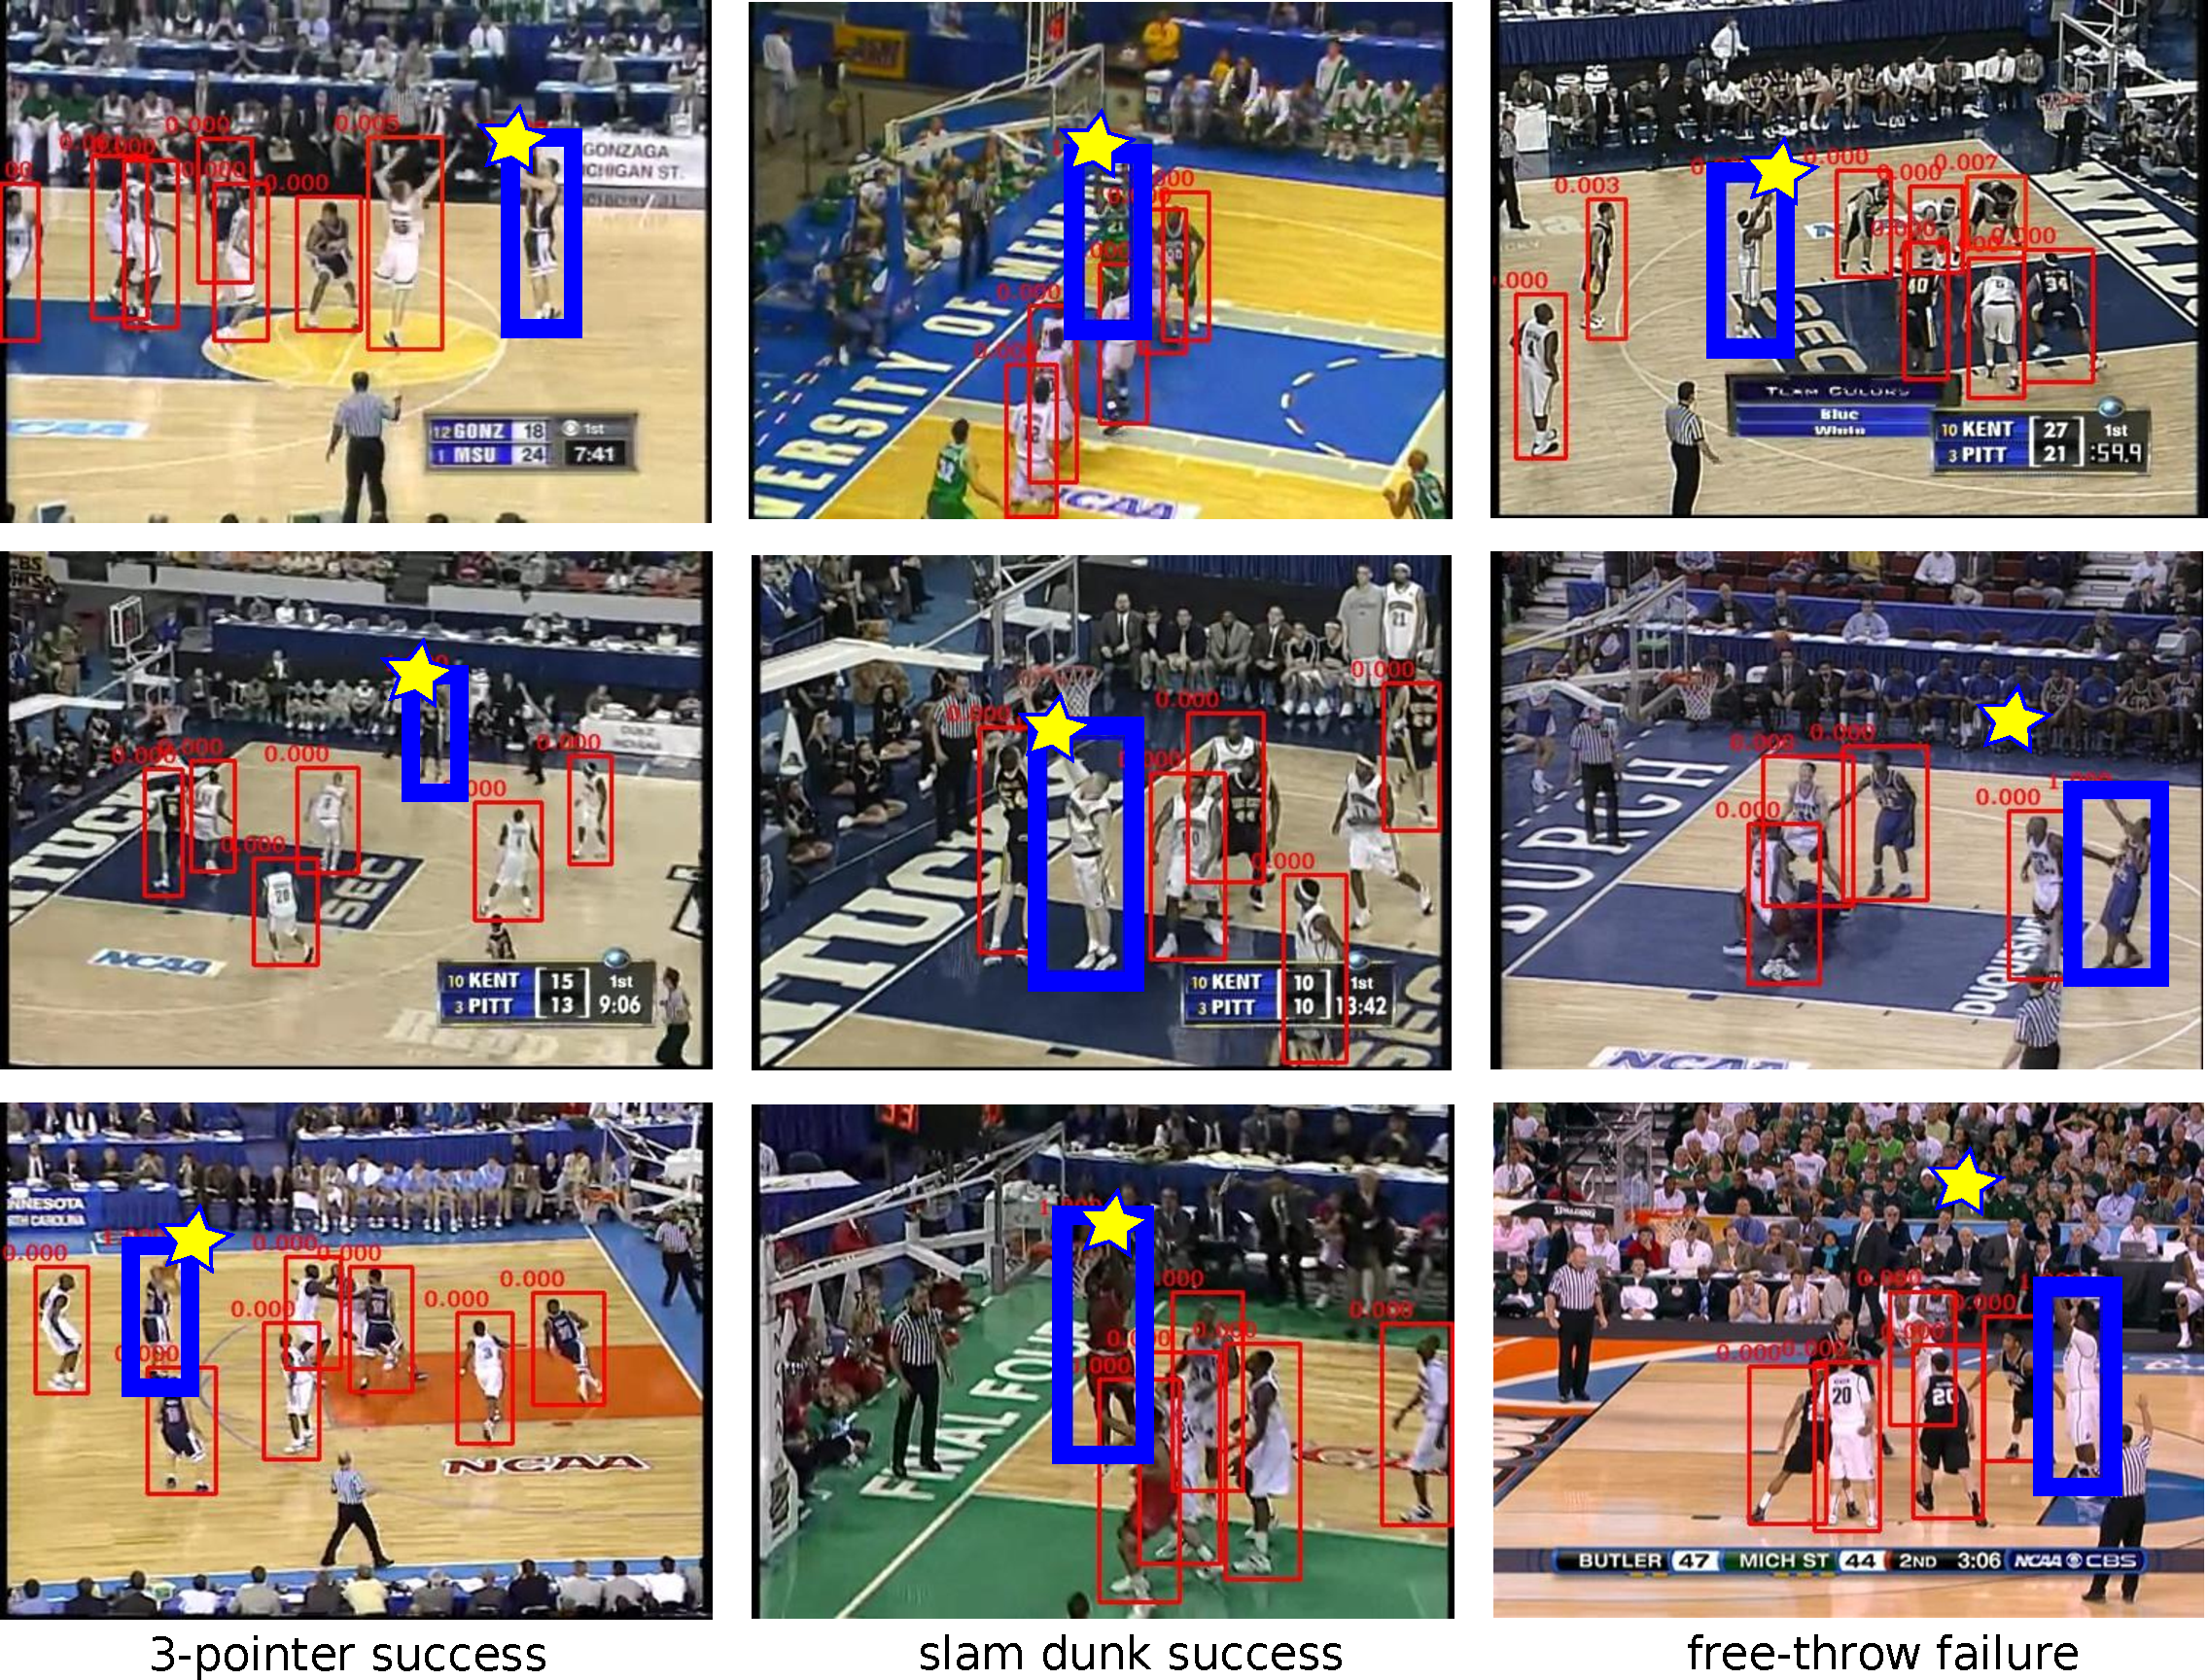
\includegraphics[width=0.90\linewidth]{images/visual_examples_v2.pdf}
\end{center}
   \caption{We highlight (in cyan) the ``attended" player at the beginning of different events.
     The position of the ball in each frame is shown in yellow.
   Each column shows a different event. In these videos, the model attends
 to the person making the shot at the beginning of the event.}
\label{fig:visual_attention}
\end{figure*}
% ---------------------------------------------------------------------------------

% -------- Heat Map for youtube videos
\begin{figure*}[t!]
\begin{center}
  \vspace{-7mm}
%  \includegraphics[width=7 in]{images/attention_heatmap_full.pdf}
  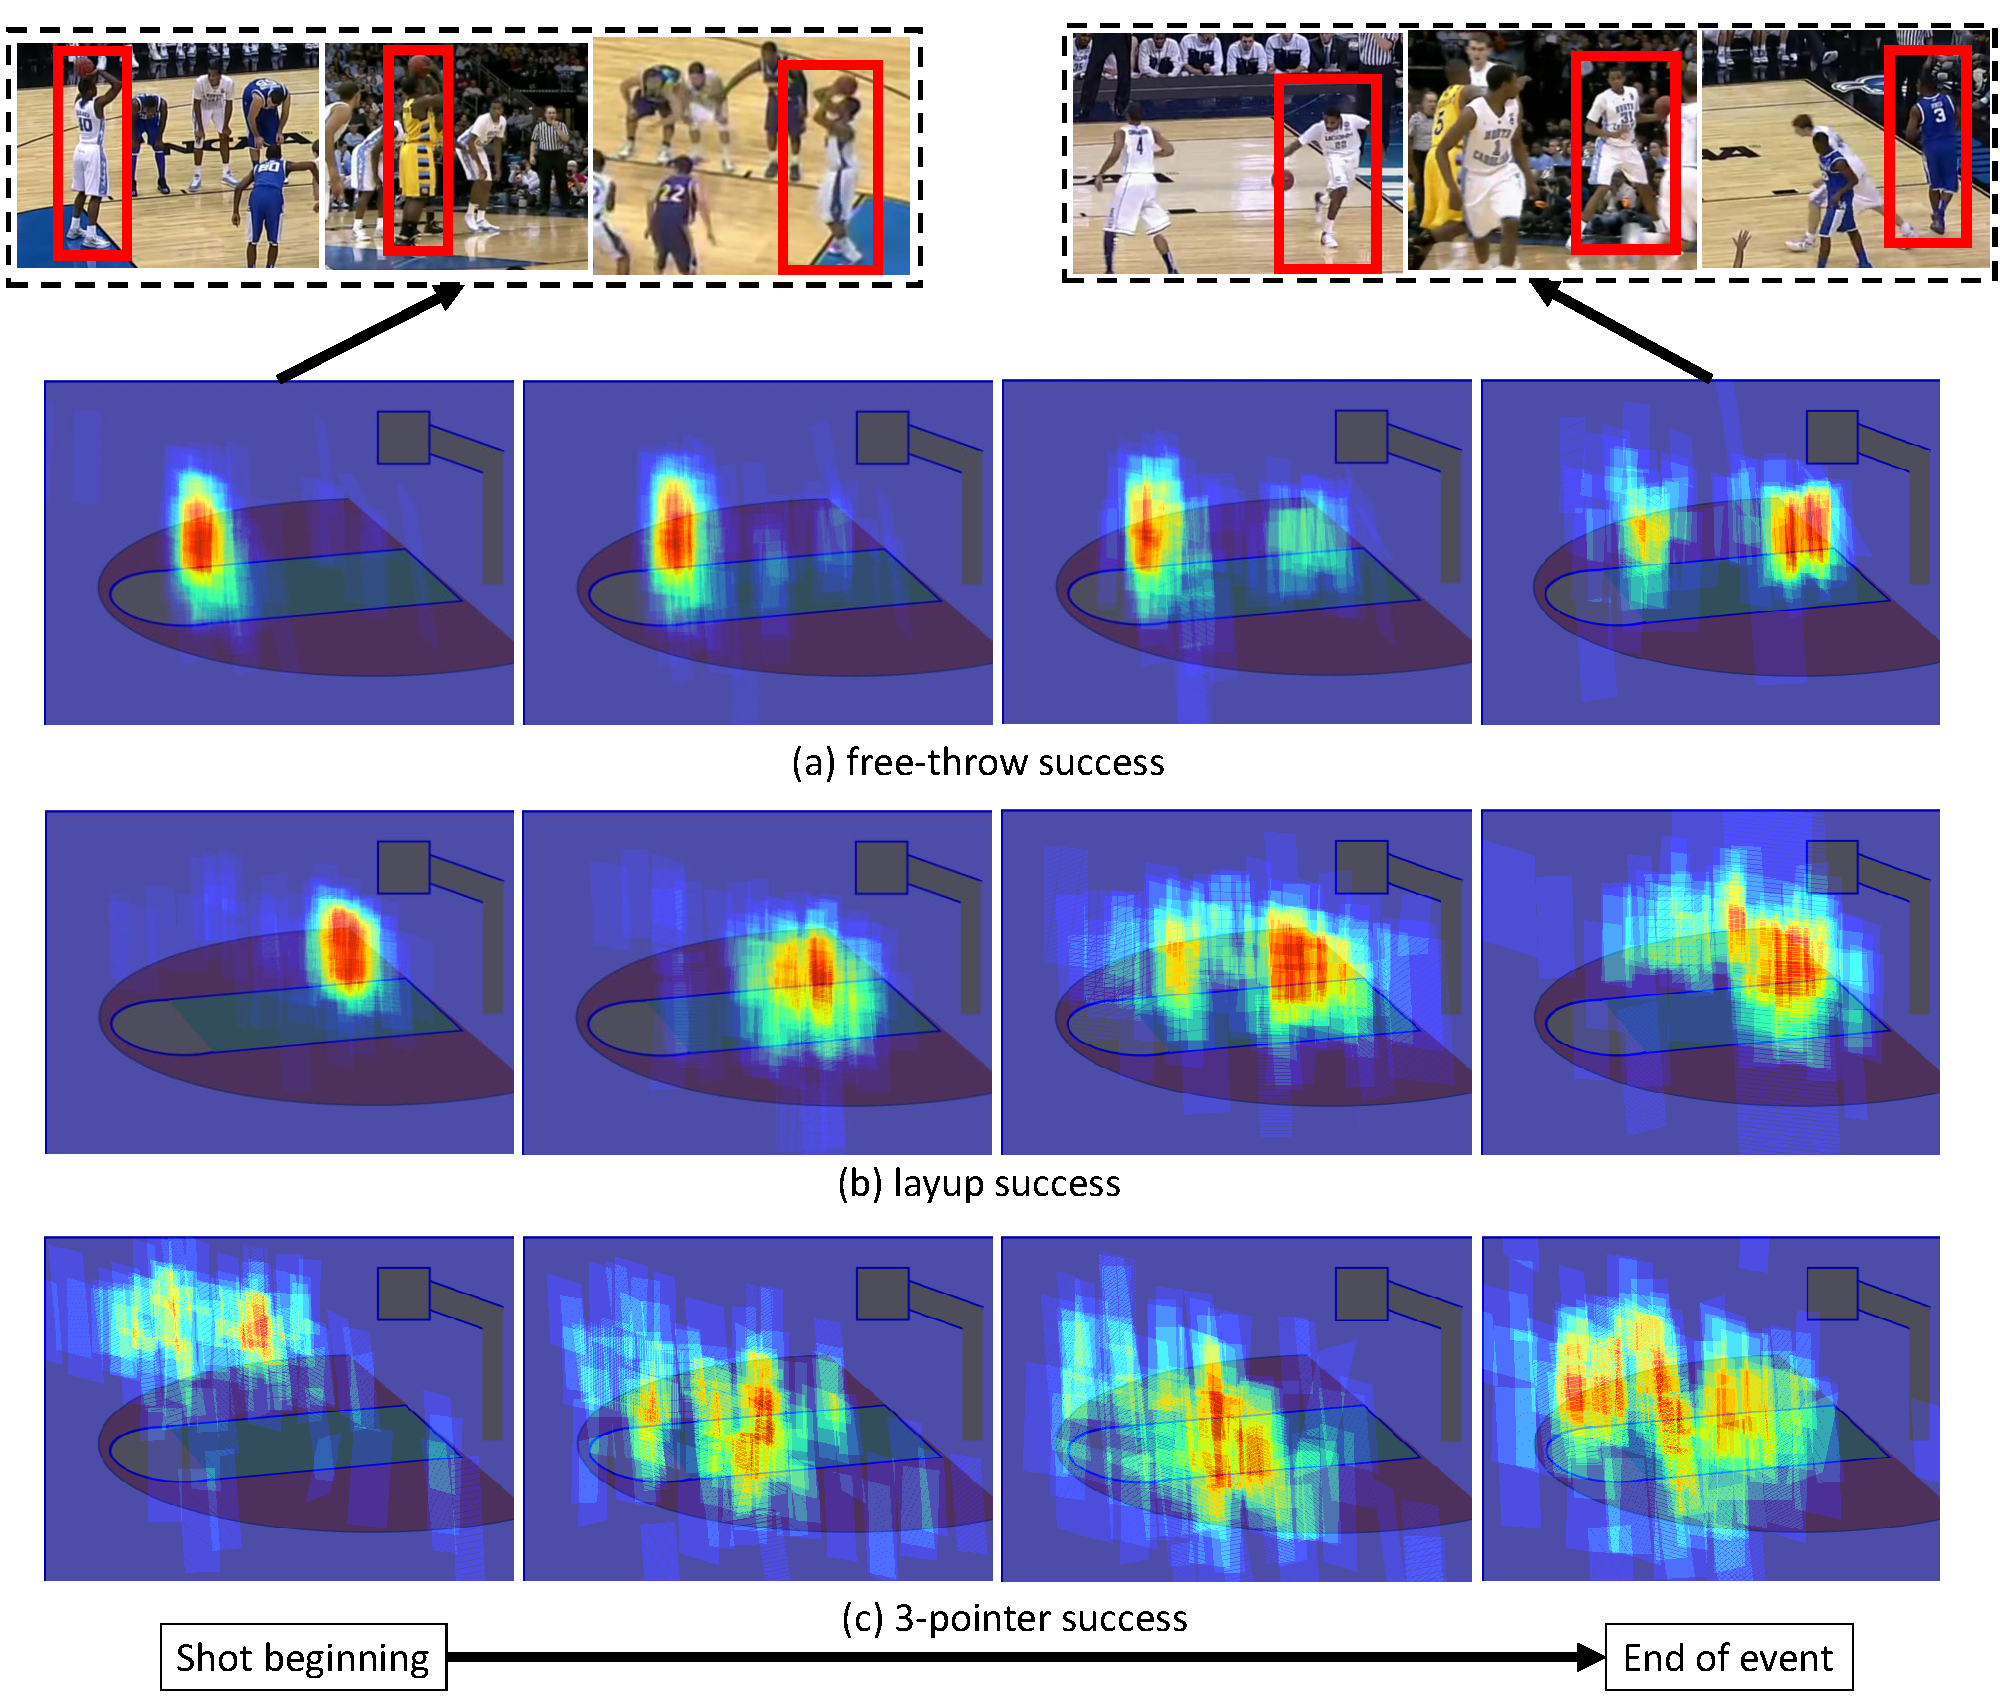
\includegraphics[width=0.9\linewidth]{images/heatmap_figure_v2_cropped.pdf}
\end{center}
  \vspace{-4mm}
   \caption{We visualize the distribution of attention over different positions of
   a basketball court as the event progresses. This is shown for 3 different events.
   These heatmaps were obtained by first transforming all videos
 to a canonical view of the court (shown in the background of each heatmap). The top row shows
 the sample frames which contributed to the ``free-throw" success heatmaps. It is interesting
 to note that the model focuses on the location of the shooter at the beginning of an
 event and later the attention disperses to other locations.}
  \vspace{-4mm}
\label{fig:att_heatmap}
\end{figure*}
% ---------------------------------------------------------------------------------

To evaluate the attention models, we  labeled the player who was
closest (in image space) to the ball as the ``shooter''.
(The ball location is annotated in 850 test clips.)
We used these annotations to evaluate if our ``attention" scores
were capable of classifying the ``shooter" correctly in these frames.

\begin{table}[ht!]
\begin{center}
\small
 \begin{tabular}{|l|c|c|c|}
  \hline
Event            & Chance & Attn. with track & Attn. no track \\ \hline \hline
3-point succ.    & 0.333 & 0.445 & 0.519 \\ 
3-point fail.    & 0.334 & 0.391 & 0.545 \\ 
free-throw succ. & 0.376 & 0.416 & 0.772 \\ 
free-throw fail. & 0.346 & 0.387 & 0.685 \\  
layup succ.      & 0.386 & 0.605 & 0.627 \\ 
layup fail.      & 0.382 & 0.508 & 0.605 \\ 
2-point succ.    & 0.355 & 0.459 & 0.554 \\ 
2-point fail.    & 0.346 & 0.475 & 0.542 \\ 
slam dunk succ.  & 0.413 & 0.347 & 0.686 \\ 
slam dunk fail.  & 0.499 & 0.349 & 0.645 \\ \hline \hline  
Mean             & 0.377 & 0.438 & 0.618 \\ \hline
  \end{tabular}
\end{center}
  \caption{Mean average precision for attention evaluation.}
  \vspace{-4mm}
  \label{tab:attention_res}
\end{table}


The mean AP for this ``shooter"  classification is listed in
Tab.~\ref{tab:attention_res}.  The results show that the track-free attention
model is quite consistent in picking the shooter for several classes like
``free-throw succ./fail", ``layup succ./fail." and ``slam dunk succ.". This is
a very promising result which shows that attention on player detections alone
is capable of localizing the player making the shot. This could be a useful cue
for providing more detailed event descriptions including the identity and
position of the shooter as well.

% -------- Heat Map for youtube videos
\begin{figure}[ht!]
\begin{center}
   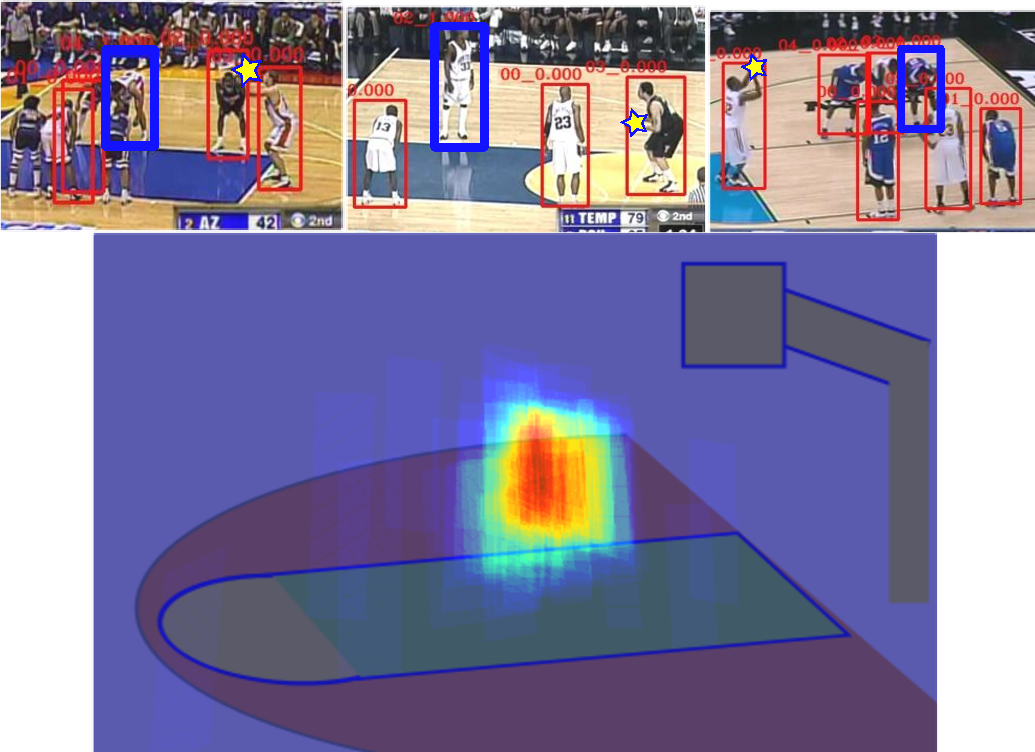
\includegraphics[width=0.9\linewidth]{images/track_spec_output.pdf}
\end{center}
  \vspace{-4mm}
\caption{The distribution of attention for our model with tracking,
     at the beginning of ``free-throw success". Unlike
     Fig.~\ref{fig:att_heatmap}, the attention is concentrated at a specific
     defender's position. Free-throws have a distinctive defense formation, and
   observing the defenders can be helpful as shown in the sample images in
 the top row.} \eat{While the model does not choose the shooter in this case, it
 consistently attends to another relevant player.}
  \vspace{-4mm}
\label{fig:visual_attention_trackspec}
\end{figure}
% ---------------------------------------------------------------------------------

In addition to the above quantitative evaluation, we wanted to visualize the
attention masks visually.  Figure~\ref{fig:visual_attention} shows 
sample videos.  In order to make results comparable across frames, we annotated
5 points on the court and aligned all the attended boxes for an event to one
canonical image.  Fig.~\ref{fig:att_heatmap} shows a heatmap  visualizing the
spatial distributions of the attended players with respect to the court. It is
interesting to note that our model consistently focuses under the basket for a
layup, at the free-throw line for free-throws and outside the 3-point ring for
3-pointers.

Another interesting observation
%from Tab.~\ref{tab:attention_res}
is that the attention scores for the tracking based model are less selective in
focusing on the shooter.  We observed that the tracking model is often
reluctant to switch attention between frames and focuses on a single
player throughout the event. This biases the model towards players who are
present throughout the video. For instance, in free-throws
(Fig.~\ref{fig:visual_attention_trackspec}) the model always
attends to the defender at a specific position, who is visible throughout the
entire event unlike the shooter.

\vspace{-2mm}
